\documentclass[10pt,conference,compsocconf]{IEEEtran}

\usepackage{hyperref}
\usepackage{graphicx}	% For figure environment

% for text in math mode
\usepackage{amsmath}

% for table
\usepackage{tabu}
\usepackage{tabularx}
\usepackage{multirow}

\begin{document}
\title{Higgs Boson Machine Learning Challenge}

\author{
  Cheng Chun Lee, I Made Sanadhi Sutandi, Haziq Razali\\
  \textit{School of Computer and Communication Science, EPFL}
}

\maketitle

\begin{abstract}
  The discovery of the Higgs-Boson in 2012 was a major breakthrough in particle physics and it was the combination of effort by inter-discipline join of physicists and data scientists, as an attempt to better understand this particle. In this paper, we tackle the problem of identifying the Higgs-Boson through the implementation of machine learning techniques. We investigate the usage of linear models to discriminate between the Higgs-Boson (signal) and background. Coupled with data analysis, we show the efficacy of our pipeline on the Higgs-Boson dataset with promising results.
\end{abstract}

\section{Introduction}

The Higgs-Boson is the first elementary particle discovered in nature through experiments at the Large Hadron Collider. Our aim in this project is to develop a learning system capable of identifying the Higgs-Boson given its decay signature. To achieve this, we use the CERN's public dataset consists of 250,000 observations, each with a vector of 30 features representing  the decay signature of a collision event. The observations are labeled 1 for an actual event and -1 for background noise.

\section{Pre-processing} 

\subsection{Data partitioning}

Initial exploratory data analysis reveals an interesting structure within the dataset: that there are several features that tightly couped by the value of PRI\_JET\_NUM (feature 22). The number of jet emissions, ranging from 0 to 3, dictate the availability of specific readings with outliers value of being designated the integer -999. It would thus make sense to posit that the number of jets emitted will result in different readings of features. Consequently, we partitioned the dataset into 4 disjoint subsets according to the emission count, removing all missing entries including the jet number. In addition to this partitioning, we also figure out that the predicitons most probably are background noises if outliers are present in DER\_MASS\_MMC (feature 1). Therefore we split each subset again into two subsets based on the presence of outliers in this feature, giving us 8 subsets in total accordingly.

\subsection{Features Removal}
We plot of a histogram of all variables and split according to the observation (signal/background). Then we find that the variables 'phi' to have no distinct pattern (Figure 1). We thus suspect that these variables do not provide useful information and decide to remove all phi related variables from the dataset.

\begin{figure}[t]
\begin{center}
  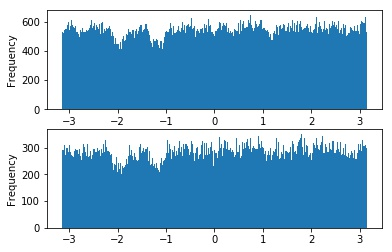
\includegraphics[width=\columnwidth]{feature.jpg}
  \caption{Histogram of the variable PRI\_lep\_phi for true observations (top) and background (bottom).}
\end{center}
   \label{fig:phi}
\end{figure}

\subsection{Feature Expansion}
Next, we augment all 8 feature matrices with non-linear transformations of the raw data to increase the expressive power of our models. More specifically, for each matrix ${\textbf X_i}$ we concatenate as follows:
\vspace*{-1mm}
\begin{equation}
{\textbf X} \leftarrow \big[ \ {\textbf X} \ \vert \ {\textbf A} \ \vert \ {\textbf B} \ \vert \ {\textbf C} \ \vert \ {\textbf d} \ \vert \ {\textbf E} \ \vert \ {\textbf F} \ \big]
\end{equation}
\vspace*{-5mm}
\begin{equation}
a_{ij} = x_{ij}^2, \ \ b_{ij} = \log (1 + x_{ij}), \ \ c_{ij} = b_{ij}^{-1}, \ \ d_{i} = 1 
\end{equation}
\vspace*{-5mm}
\begin{equation}
E = (X)*(X), \ \ f_{ij} = \sqrt{x_{ij}}
\end{equation}

bringing the size of each matrix from $ (N \times m_i) $ to $ (N \times (4m_i + 1))$. A drawback of feature augmentation is the increased tendency for models to overfit which we can reduce via regularization. Note that we have also append a column vector of ones to the final matrix to act as the bias term present in linear models. 

\begin{figure*}[t]
\begin{center}
  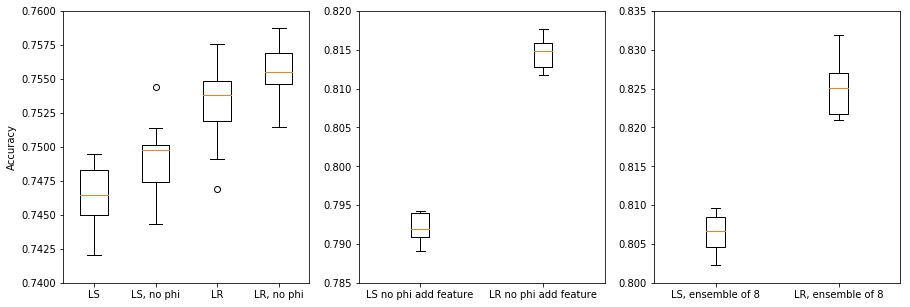
\includegraphics[width=\textwidth]{box1.jpg}
  \caption{Box plot distributions of our models.}
\end{center}
   \label{fig:boxplot}
\end{figure*}

\subsection{Standardization}
Learning algorithms often benefit from the many standardization techniques to prevent any particular feature from dominating the objective function. In our implementation, we standardize our data using standard score (z-score) normalization in which by scaling each feature to have zero-mean and unit-variance.

\section{Models}

We experiment with the following linear models: Least Squares and Logistic Regression with $L_2$ regularization. All weights are initialized by sampling from a normal distribution with zero-mean and unit variance. Recall from section II that the data was split into 8 subsets; our algorithm thus builds 8 separate classifiers trained on each subset. Since we define 5000 iterations for each subset, we use small value of step-size of 0.000002 in order to best compromise between stability and time. Smaller step size ensures we osiciliate closely to the global minimum. We then train all models using gradient descent with a total of 5000x8 iterations (a pass through the entire dataset). We list all parameters in Table 1. At test time, we simply process the input data as described in section II and select the appropriate classifier for discrimination.

\begin{table}[t]
 	\small
	\begin{tabu} to \columnwidth { | X[l] | X[c] | X[0.9c] |}
	    \hline
		\multirow{2}{*}{\textbf{Dataset}} & \multicolumn{2}{c|}{\textbf{Accuracy (\%) }} \\
		\cline{2-3}
		& Logistic Regression & Least Squares \\
		\hline
		Jet 0 with mass & 80.836 & 80.458 \\
		\hline
		Jet 0 without mass & 95.050 & 95.035 \\
		\hline
        Jet 1 with mass & 79.499 & 78.312 \\
		\hline
        Jet 1 without mass & 92.290 & 92.542 \\
		\hline
        Jet 2 with mass & 83.526 & 82.187 \\
		\hline
        Jet 2 without mass & 92.107 & 92.988 \\
		\hline
        Jet 3 with mass & 82.675 & 81.476 \\
		\hline
        Jet 3 without mass & 94.177 & 96.208 \\
		\hline
        Ensemble & - & - \\
		\hline
		\end{tabu}
	\medskip
	\caption{The accuracies of each component in the ensemble along with their aggregated scores}	
\end{table}

\section{Experiments}

We evaluate the above-mentioned models on the Higgs-Boson dataset using 10-fold cross validation. Since we perform several pre-processing steps, it is reasonable to evaluate how much the overall result depends on each component. In our first experiment, we study the improvements obtained when we gradually append additional steps in our pre-processing pipeline. Summarized in Figure 2 are the box-plot distributions of our models, each with additional components gradually added. Note that the figures on the left and middle display the results when using only a single classifier i.e. we do not partition the data as described in 2A. Also note that their features have been standardized taking only non missing entries into account with these entries then set to 0. The figure on the right display the results of the complete system as discussed in previous sections.

These results show fascinating studies. Firstly, we see that both models trained on the standardized raw-data are quite close in their prediction accuracy. The removal of all phi-related features provides a small boost in performance. The figure also clearly illustrates the improvements obtained when training the models on the augmented feature matrix with an approximate increase of 4\% in the accuracy of both classifiers, suggesting the presence of a non-linear decision boundary. Lastly, we can observe that training an ensemble of classifiers on the 8 subsets has a positive influence on the overall performance. 

We then measure the performance of each component in the ensemble and their overall accuracy, weighted by the size of the subsets. It is interesting to see that the classifiers for datasets without mass have higher accuracy, although we have already found that these datasets have a majority of their observations labeled as background. 

From all the experiments, we note that the least squares classifier lags behind the logistic in terms of accuracy. This is most likely due to the cost function in least squares that renders it less resilient against outliers. Lastly, the deviations in the accuracy also implies that the classifiers did not over-fit the training data.

\section{Conclusion}

We have presented a technique for identifying the Higgs-Boson. Our system employs an ensemble of 8 classifiers that heavily relies on feature processing. We saw in the previous section that the largest improvement is obtained when we map the features into a higher dimensional space. Possible extensions can thus incorporate the use of highly non-linear classifiers such as neural networks. The inclusion of domain specific feature engineering could also prove worthwhile.

\bibliographystyle{IEEEtran}
\bibliography{literature}

\end{document}
